\JWlone{Design}
\label{sec:design}


%#  BIG PICTURE  ###############################################################
\JWltwo{Big Picture of the Setup}
\label{sec:big-pic}

\begin{figure}
  \centering
    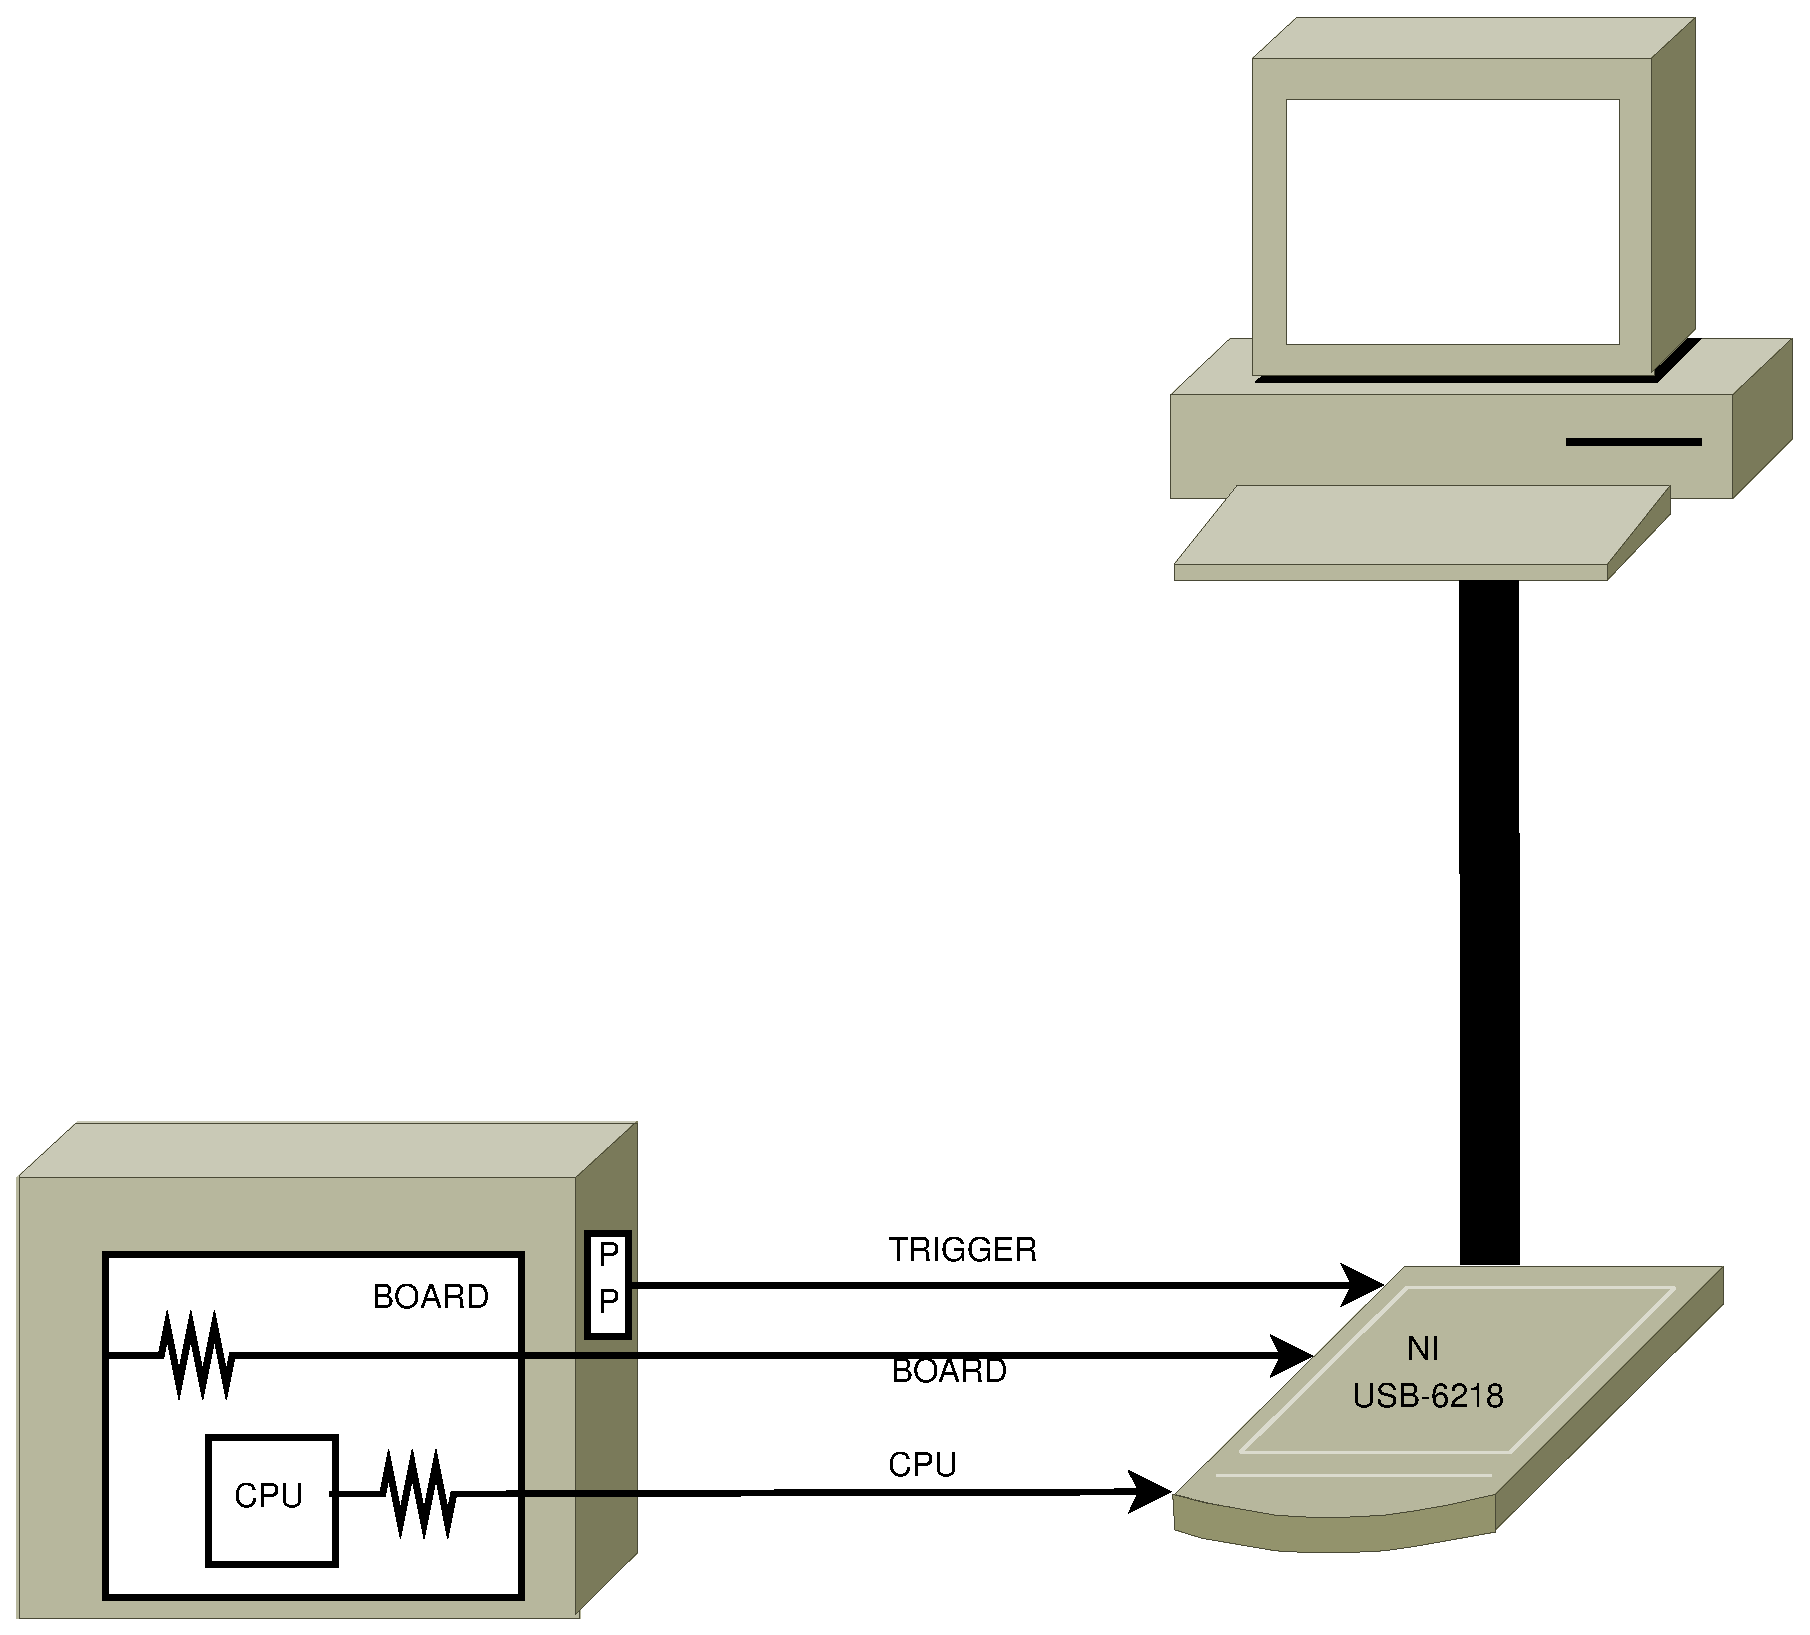
\includegraphics[width=\textwidth]{fig/measuring-overview.eps}
  \caption{Measuring setup overview}
  \label{fig:overview}
\end{figure}

As figure \ref{fig:overview} illustrates, an additional workstation---the
\emph{Examining Workstation (EW)}---has been used while evolving this thesis.
The \emph{System under Test (SuT)} counts the CPU's performance events itself
and the EW records the energy consumption using a measuring device in the
meantime. The resulting data sets have thereafter been used to build up the
energy model.


%#  MEASURING SETUP IN DETAIL  #################################################
\JWltwo{Measuring Setup in Detail}
\label{sec:measuring-setup}

To fit the energy model afterwards, the current flows of the CPU and the
motherboard's \SI{12}{\volt} supply have to be measured. Voltage drops across
the sensing resistor are measured using four--terminal sensing \cite{wiki:FTS}
to deduce the current flow. The motherboard's \SI{12}{\volt} current flow has
been measured in this thesis because it was unclear if the CPU is entirely fed
by its own \SI{12}{\volt} power supply.

Because the SuT and the EW (see figure \ref{fig:overview}) have to agree about
the examination (time) interval a trigger wire is used. It is realized as a
simple analog signal using the parallel port's \emph{high} and \emph{low}
voltages.

This can be summed up to measure three potential differences. Since the
measuring device (chapter \ref{sec:measuring-device}) provides up to eight
differential, analog input channels this seems easy at first. Unfortunately,
two caveats apply: On the one hand according to the user's manual
\cite{NIManual2009} the best measuring accuracy can be achieved in range of
\SI{-200}{\milli\volt} and \SI{200}{\milli\volt}. On the other hand the overall
potential differences may not exceed $\pm$\SI{10.4}{\volt} \cite{NISpec2009}.

\begin{figure}
  \centering
    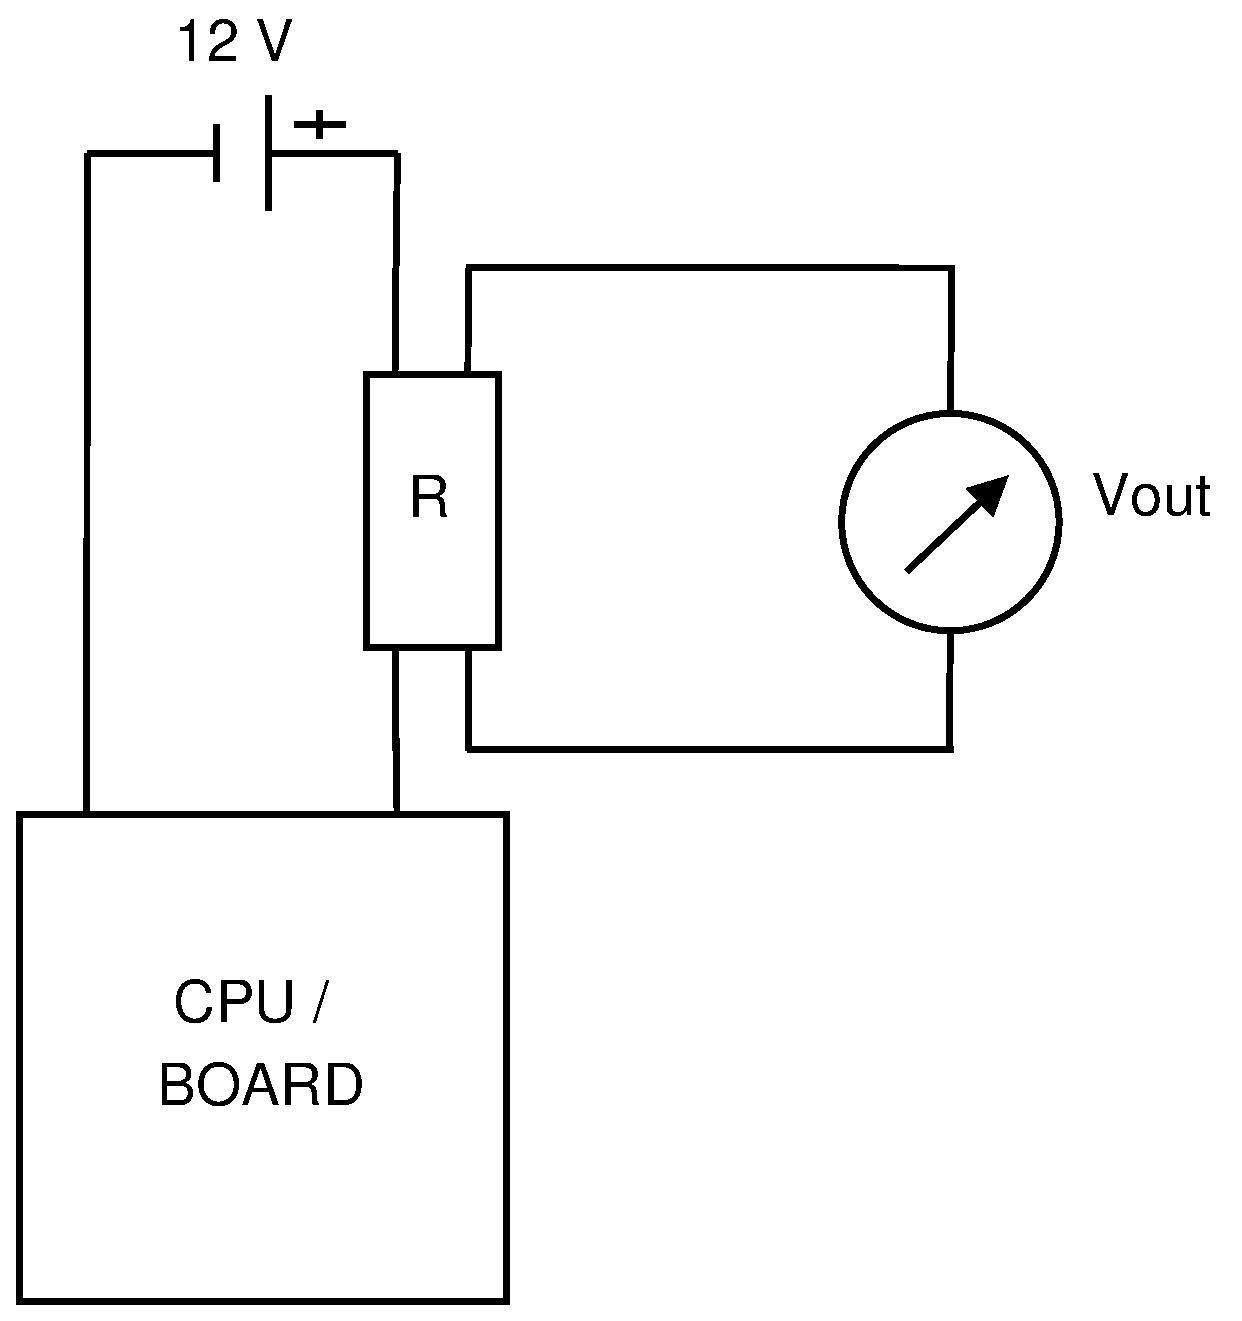
\includegraphics[width=0.5\textwidth]{fig/measuring-circuit.eps}
  \caption{Measuring circuit for CPU (R=\SI{10}{\milli\ohm}) and BOARD
(R=\SI{5}{\milli\ohm})}
  \label{fig:circuit}
\end{figure}

\begin{figure}
  \centering
    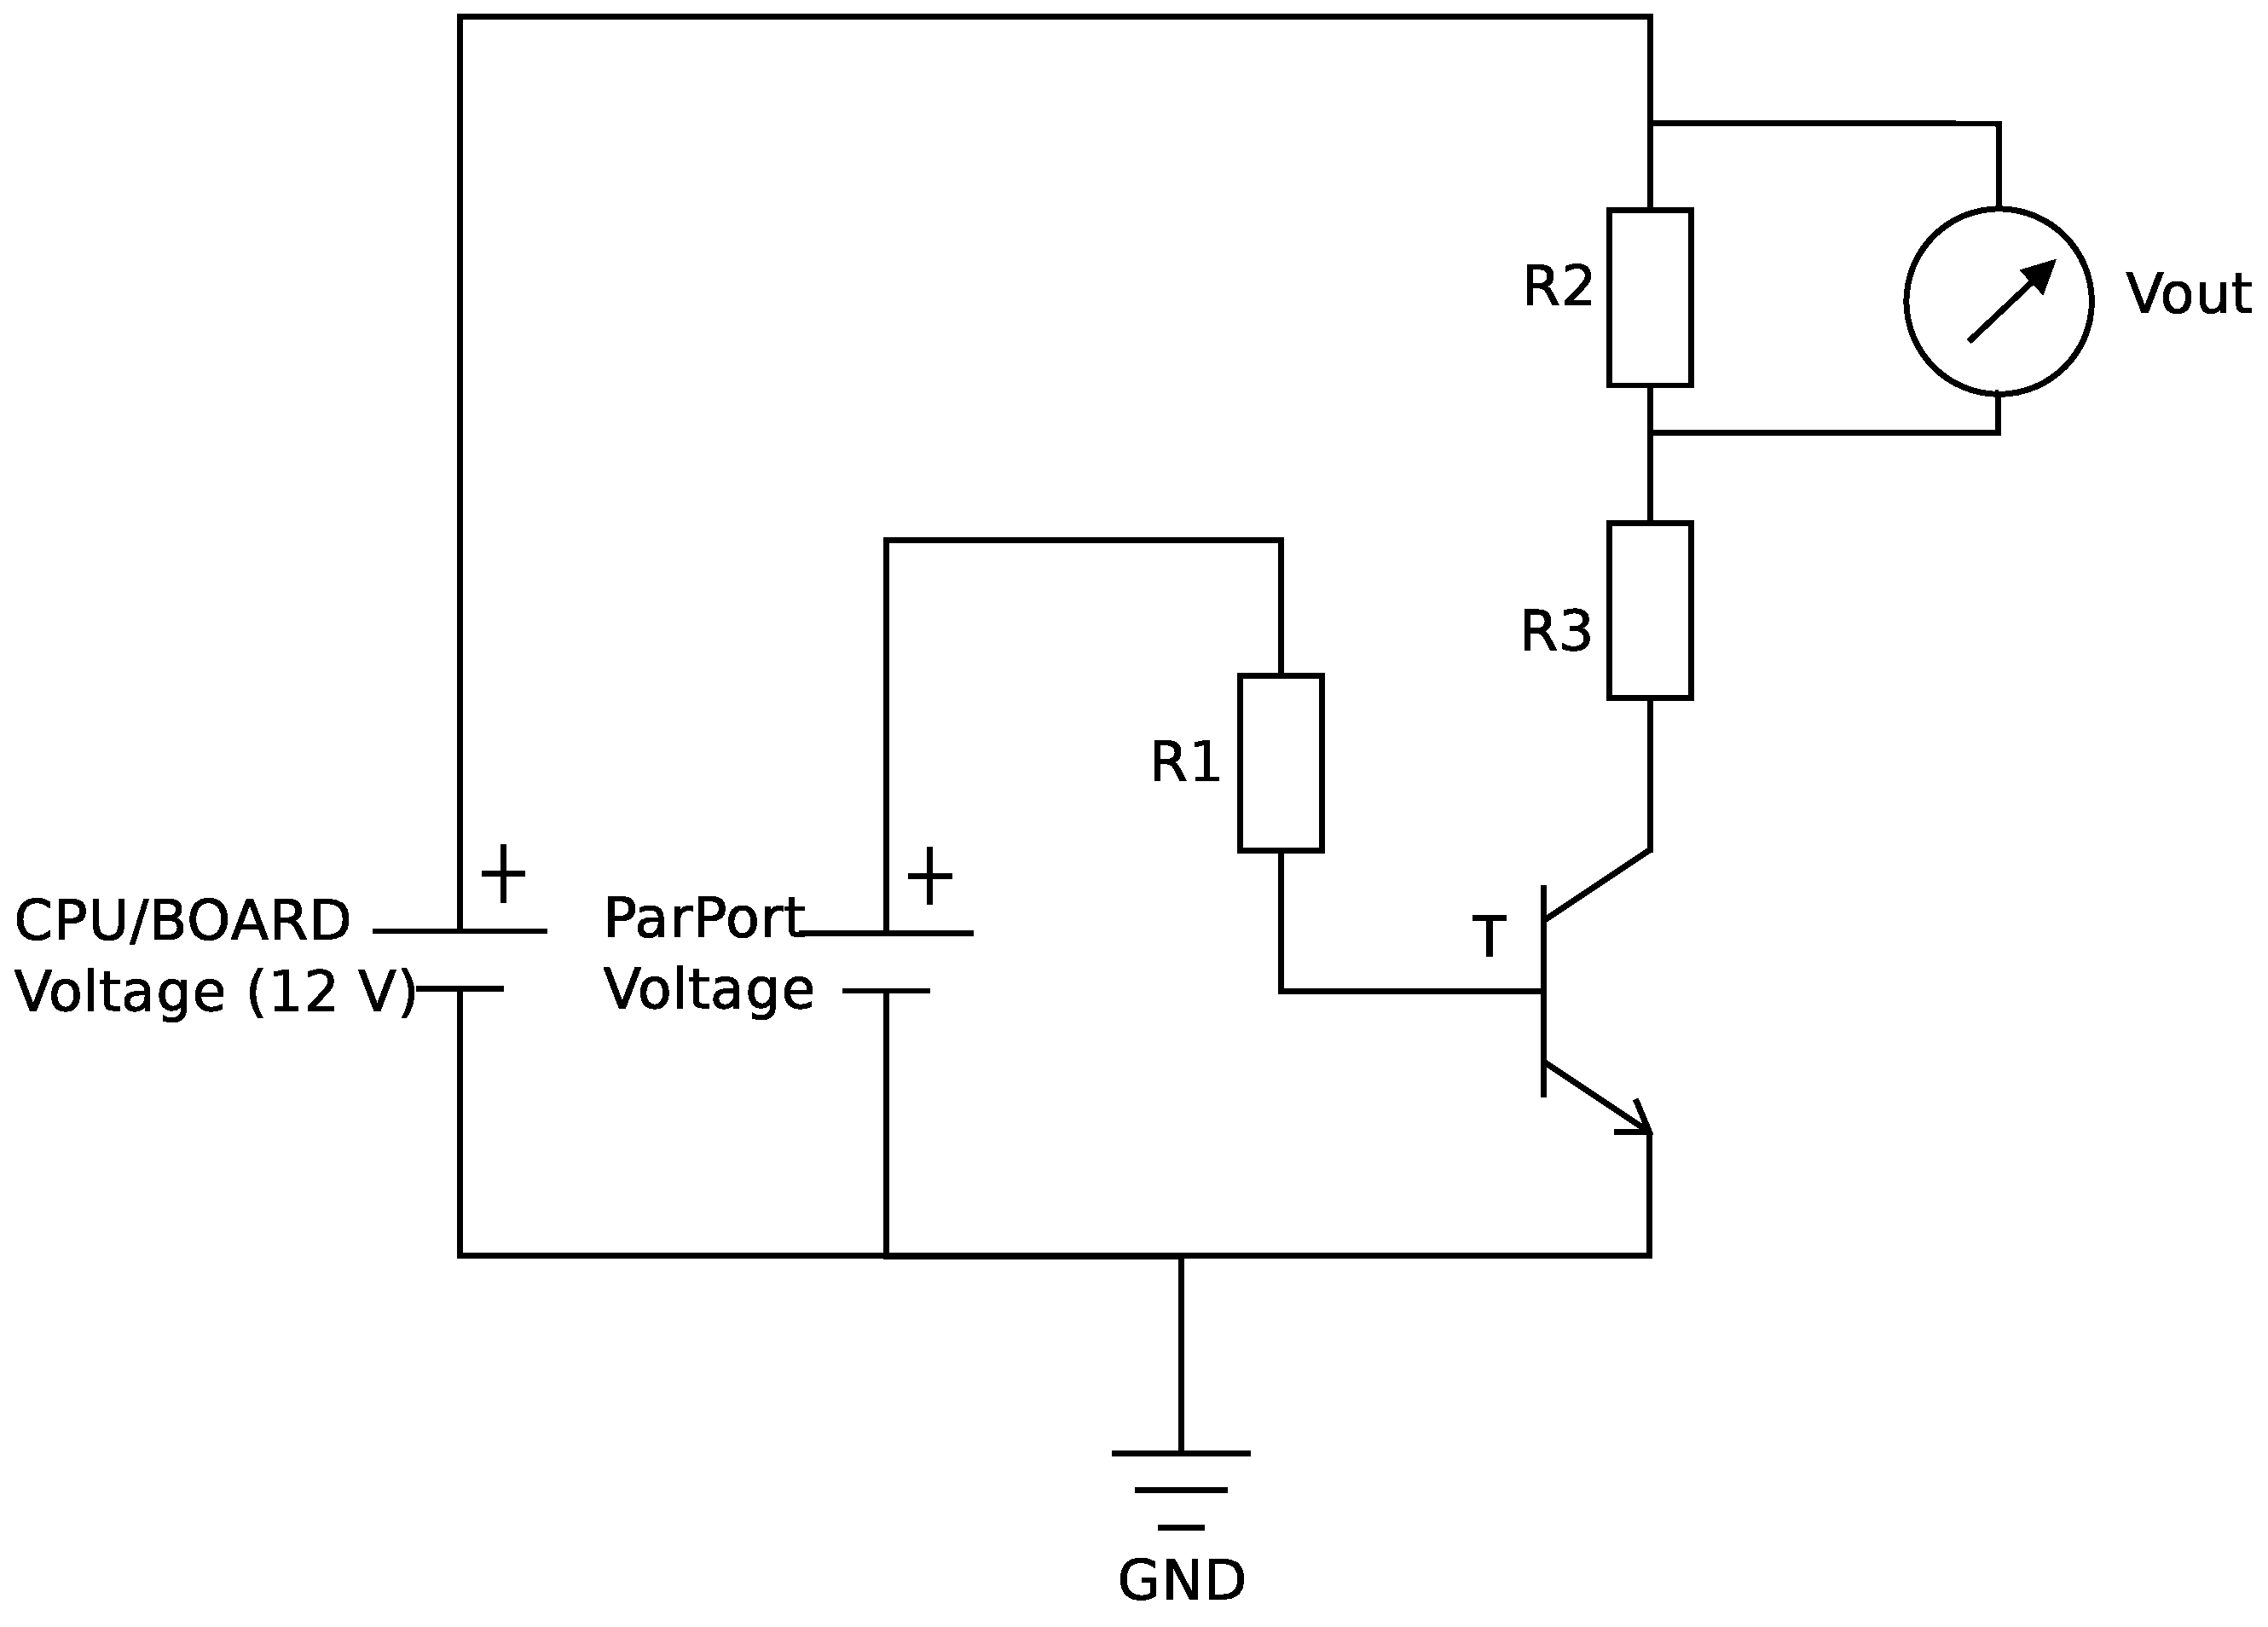
\includegraphics[width=\textwidth]{fig/potential-equalizer.eps}
  \caption{Potential equalizer}
  \label{fig:potential-equalizer}
\end{figure}

Choosing adequate sensing resistors for the \JWchan{CPU} (R =
\SI{10}{\milli\ohm}) and \JWchan{BOARD} (R = \SI{5}{\milli\ohm}) channels (see
figure \ref{fig:circuit}) worked out well. The parallel port trigger wire has
been a problem at first, though. The parallel port has a potential difference
range of more than \SI{200}{\milli\volt} and our test machine's port had a very
different potential level than the \JWchan{CPU} and \JWchan{BOARD} channels,
exceeding the allowed range of $\pm$\SI{10.4}{\volt}.  The potential equalizer
illustrated in figure \ref{fig:potential-equalizer} solves both problems.

Finally, three differential channels \JWchan{CPU}, \JWchan{BOARD}
(\SI{12}{\volt} supply only!) and \JWchan{TRIGGER} in the range of
$\pm$\SI{200}{\milli\volt} and alike potential levels can be connected to the
measuring device. The performance events get counted on the SuT itself which
controls the trigger wire, too: The trigger is set to \emph{On} directly before
executing the program to examine and is set to \emph{Off} promptly after its
termination. To safely register all CPU energy consumption peaks, a high
sampling rate of \SI{50}{\kilo\samples\per\second} is chosen. An exemplary
plot of an examination can be found in figure \ref{fig:cpu-power-trig}.

\begin{figure}
  \centering
    \includegraphics[width=\textwidth]{fig/cpu-power-trig.eps}
  \caption{Sample examination}
  \label{fig:cpu-power-trig}
\end{figure}


%-  measuring device  ----------------------------------------------------------
\JWlthree{Measuring Device}
\label{sec:measuring-device}

For measuring the voltage drops a \JWPLni{} from
\JWenterprise{http://www.ni.com}{National Instruments} (shown in figure
\ref{fig:ni}) was chosen because its support for high sampling rates of up to
250000 samples per second (\SI{250}{\kilo\samples\per\second}) and its high
accuracy (accuracy $< \SI{2.69}{\milli\volt}$)\cite{NISpec2009}.

\begin{figure}
  \centering
    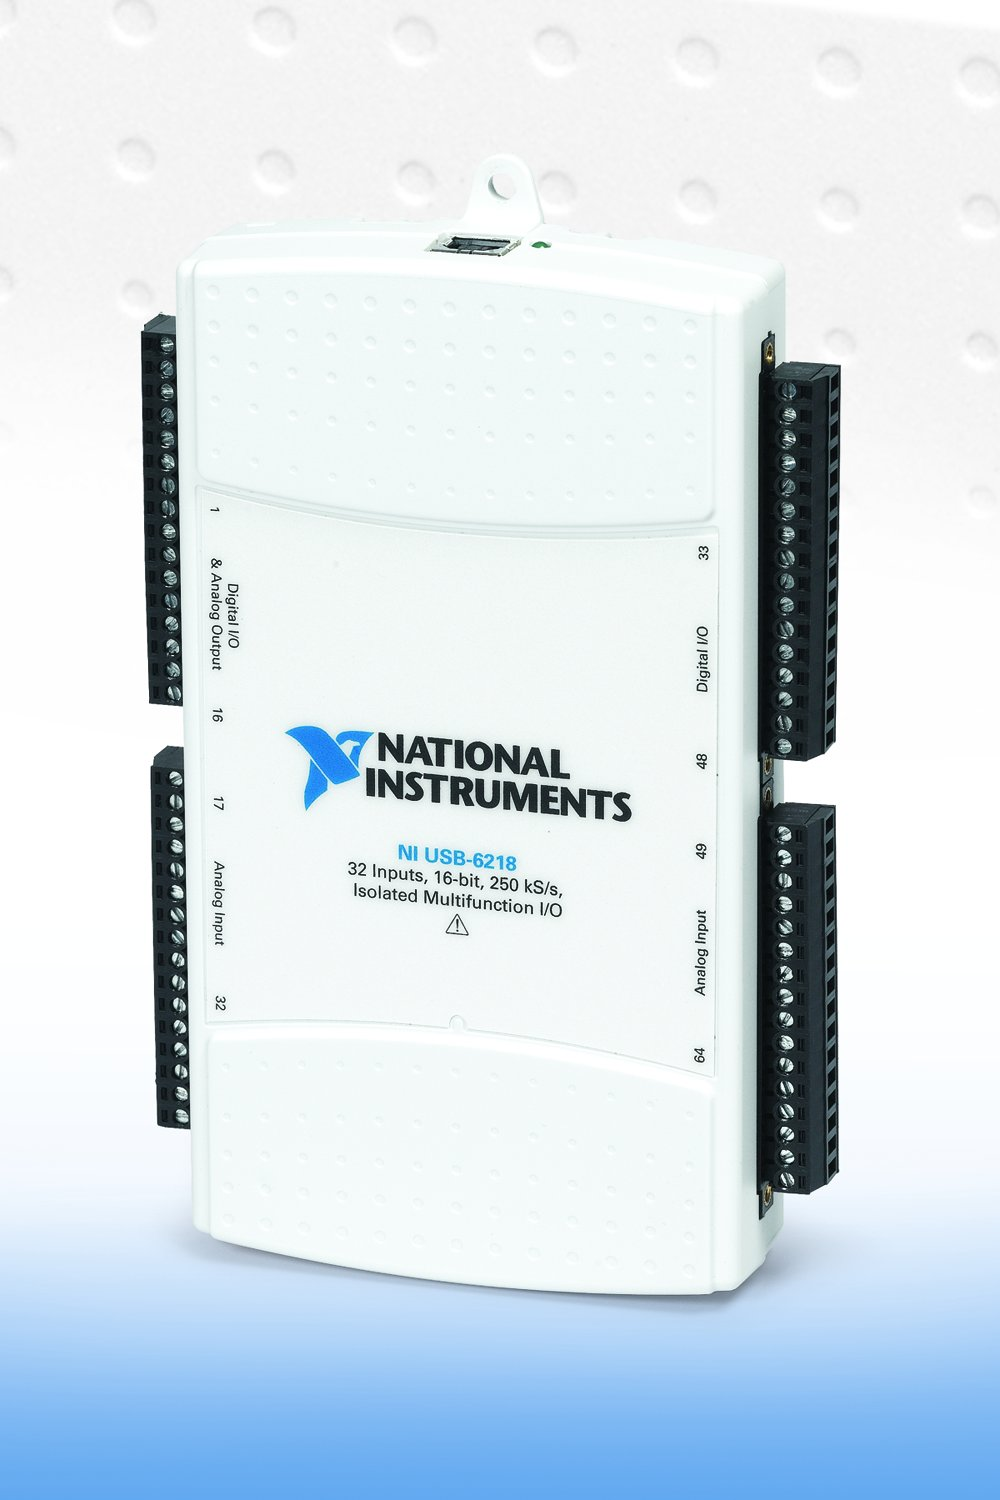
\includegraphics[width=0.5\textwidth]{fig/NI-USB-6218.jpg}
  \caption{\JWPni{} (picture from \JWlink{http://www.pressebox.de/pressemeldungen/national-instruments-germany-gmbh/boxid/75241})}
  \label{fig:ni}
\end{figure}


%#  CALCULATION OF THE ELECTRICAL WORK  ########################################
\JWltwo{Calculation of the Electrical Work}
\label{sec:calc-work}

From elementary physics (resistance $R$, voltage $U$, electric current $I$ and
instantaneous electric power $P$):

\begin{eqnarray}
     U = R * I \iff I = \frac{U}{R} \\
     P = U * I
\end{eqnarray}

So, the current flow is calculable from the voltage drops across the
measuring resistor ($U_R$). Accordingly, the instantaneous power can be
calculated as:

\begin{eqnarray}
P & = & U * I \\
  & = & U * \frac{U_R}{R} \\
P & = & \frac{12V * U_R}{R}
\end{eqnarray}

Hence, integrating will result in the electrical work

\begin{equation}
  W = \int P(t)dt
\end{equation}


%#  ENERGY MODEL  ##############################################################
\JWltwo{The Energy Model}
\label{sec:model}

The following chapters will define the term \emph{energy model} along with  the
formal methods suggested to build such a model.


%-  the model's properties  ----------------------------------------------------
\JWlthree{Properties}
\label{sec:model-properties}

In this work, an energy model is considered as a linear function. It describes a
system with $n_c$ cores that is able to monitor $n_e$ performance events per
core simultaneously. Additionally to the per--core event counters,
$n_g$ global event counters make the model up. In the formal description (see
chapter \ref{sec:towards-the-model} for the practical implementation) we assume
four functions providing the actual values:

\begin{itemize}

\item $c_g(i, t_0, t_e) \in \mathbb{N}^{\{1, \ldots, n_e\} \times
\mathbb{R}_{\geq 0} \times \mathbb{R}_{\geq 0}}$, the global event $i$'s count
in the time interval $(t_0, t_e)$

\item $c_e(j, k, t_0, t_e) \in \mathbb{N}^{\{1, \ldots, n_c\} \times
\{1, \ldots, n_g\} \times \mathbb{R}_{\geq 0} \times \mathbb{R}_{\geq 0}}$, the
performance event $k$'s count on core $j$ in the interval $(t_0, t_e)$

\item $w_g(i) \in \mathbb{R}^{\{1, \ldots, n_g\}}$, the global event $i$'s
energy weight in \si{\joule}

\item $w_e(j, k) \in \mathbb{R}^{\{1, \ldots, n_c\} \times \{1, \ldots, n_g\}}$,
the weight of performance event $k$ in \si{\joule} on core $j$

\end{itemize}

Though, an energy model equates to a linear function. The function's value is
the electrical work performed between two instants of time $t_0$ and $t_e$:

\begin{equation}
W(t_0, t_e) = \sum\limits_{i=1}^{n_g} c_g(i, t_0, t_e) w_g(i) +
\sum\limits_{j=1}^{n_c} \sum\limits_{k=1}^{n_e} c_e(j, k, t_0, t_e) w_e(j, k)
\end{equation}

The functions $c_e$ and $c_g$ contain the system's live data whereas the energy
weight functions $w_e$ and $w_c$ can be calculated a priori as done in this
work. Obviously, the selection of the events and their respective weights highly
depend on the type of microprocessor. To calculate the electrical power the
system consumes, typically an arbitrary frequency $f$ (period length $T =
\frac{1}{f}$) is chosen and the variables $t_0$ and $t_e$ are set accordingly
($t_0 = ?$, $t_e = t_0 + \frac{1}{f} = t_0 + T$). The instantaneous power is
then calculated as:

\begin{eqnarray}
P(t) & = & \frac{W(t - T, t)}{T} \\
     & = & \frac{\sum\limits_{i=1}^{n_g} c_g(i, t - T, t) w_g(i) +
                 \sum\limits_{j=1}^{n_c}
                 \sum\limits_{k=1}^{n_e} c_e(j, k, t - T, t) w_e(j, k)
                }{T}
\end{eqnarray}


%-  finding the energy weights  ------------------------------------------------
\JWlthree{Finding the Energy Weights}
\label{sec:finding-weights}

Having seen what exactly constitutes an energy model (chapter
\ref{sec:model-properties}), it is crucial to find a small and significant set
of performance events and appropriate energy weights. This chapter will focus on
how to find the weights. A separate chapter (\ref{sec:min-events}) describes the
downsizing of the event set. To find reasonable energy weights test
program (also called benchmark) execution observations have to be recorded and
evaluated. Each test program run record contains the following data:

\begin{itemize}

\item $b$, the point in time the run began

\item $e$, the point in time the run ended

\item The $n_g$ values of the functions $c_g(1 \cdots n_g, b, e)$

\item The $n_c * n_e$ values of the functions
$c_e(1 \cdots n_c, 1 \cdots n_e, b, e)$

\item The electrical work $j$ the system performed between $b$ and $e$

\end{itemize}

Since the fitting of the energy weights needs a large data set, a matrix
representation is appropriate. So, $n_o$ observations in the non--overlapping
time intervals $(b_{1 \cdots n_o}, e_{1 \cdots n_o})$ lead to:

\begin{itemize}

\item $b_{1 \cdots n_o}$, the points in time the runs began

\item $e_{1 \cdots n_o}$, the points in time the runs ended

\item The matrix $Cg$ containing the global counter values (see equation
\ref{eqn:cg})

\item The matrix $Ce$, containing the performance event counter values (see
equation \ref{eqn:cc})

\item The vector $j = <j_1, \cdots, j_{n_o}>$, containing the electrical work
performed

\end{itemize}

\begin{eqnarray}
%% Cg
\label{eqn:cg}
& Cg & \in \mathbb{N}^{n_o \times n_g} \\
& Cg & =
\begin{pmatrix}
c_g(1, b_1, e_1)         & \cdots & c_g(n_g, b_1, e_1)        \\
\vdots                   & \ddots & \vdots                    \\
c_g(1, b_{n_o}, e_{n_o}) & \cdots & c_g(n_g, b_{n_o}, e_{n_o})
\end{pmatrix} \\
%% Ce
\label{eqn:cc}
& Ce & \in \mathbb{N}^{n_o \times n_cn_e } \\
& Ce & =
\begin{pmatrix}
c_e(1, 1, b_1, e_1)         & \cdots^* & c_e(n_c, n_e, b_1, e_1)         \\
\vdots                      & \ddots^* & \vdots                          \\
c_e(1, 1, b_{n_o}, e_{n_o}) & \cdots^* & c_e(n_c, n_e, b_{n_o}, e_{n_o})
\end{pmatrix}
\end{eqnarray}

$ ^*$) an arbitrary incrementation scheme---consistent with vector $w$---may be
chosen

Using a linear regression (of equation \ref{eqn:lin-reg}), suitable energy
weight vectors $w_c$ and $w_g$ can be found. The goal is to minimize the error
term, i.\,e.\ $\sum\epsilon^2$ as small as possible.

\begin{equation}
\label{eqn:lin-reg}
j = C w + \epsilon
\end{equation}

\begin{eqnarray*}
%% j
j & = &
\begin{pmatrix}
j_1 \\
\vdots \\
j_{n_o}
\end{pmatrix} \\
%% C
C & = & \big( Cg \arrowvert Ce \big) \in \mathbb{N}^{n_o \times n_g+n_cn_e} \\
& = &
\begin{pmatrix}
Cg_{1,1}   & \cdots & Cg_{1,n_g}   & Ce{1,1}   & \cdots & Ce{1,n_cn_e} \\
\vdots     & \ddots & \vdots       & \vdots    & \ddots & \vdots       \\
Cg_{n_o,1} & \cdots & Cg_{n_o,n_g} & Ce{n_o,1} & \cdots & Ce{n_o,n_cn_e} \\
\end{pmatrix} \\
%% w
w & = &
\begin{pmatrix}
w_g(1) \\
\vdots \\
w_g(n_g) \\
w_e(1, 1) \\
\vdots \\
w_e(n_c, n_e)
\end{pmatrix} \\
\end{eqnarray*}


%-  minimizing the counter set  ------------------------------------------------
\JWlthree{Minimizing the Set of Performance Events}
\label{sec:min-events}

It is not practical to take into account all events the microprocessor is aware
of. Today's processors offer much more events than they can count simultaneously
\cite{intel2011softdev1}. The function and matrix names of the previous
chapter (\ref{sec:finding-weights}) also apply here. The single exception is
that this chapter only focuses on the CPU's performance events.  The global
events are not taken into account here because they are pseudo--events not
obtained by the limited PMU and therefore have no maximal quantity.
The approach to find a subset of $n_e$ events (of $e_{max}$ available) used in
this work can be summed up to the following two steps which will be discussed in
detail later:

\begin{enumerate}

\item Generation of the matrix of performance event counters $Ce$ and
the corresponding vector of electrical works $j$

\item Obtaining $Ce_{final}$ containing the $n_e$ most correlating columns of
$Ce$ that will form the energy model's performance events

\end{enumerate}

Thereafter, the performance events the model finally uses are found. The next
step is to find the final energy weights as in the previous chapter
(\ref{sec:finding-weights}).


\JWlfour{Step 1: Generating $Ce$ and $j$}

\begin{enumerate}[(a)]

\item Choose $p$ test programs which use the CPU differently. The test
programs have to be independent from external events. We consider subsequent
runs of a test program as equal.

\item Divide the $e_{max}$ available events in $g$ disjoint, non--empty sets
$E_{1..g}$ each of size up to $n_e$.

\item For each set $E_{1..g}$, run all the $p$ test programs and record the
electrical work performed and the event counters of the set's events.

\item The electrical work of each of the runs of a test program should be
roughly equal. If they differ a lot, there is either a dependency on external
events in the benchmark or the machine is otherwisely stressed. In the former
case the test program selection should be improved, in the latter the affected
test runs have to be repeated.

\item Folding all the results leads to a vector $j \in \mathbb{R}^p$ containing
the electrical work a run of each of the test programs performed. Additionally,
a matrix $Ce$ (as in chapter \ref{sec:finding-weights}) accrues, containing each
event counter's value for a run of each of the test programs.

\end{enumerate}

\JWlfour{Step 2: Deriving $Ce_{final}$ from $Ce$}

\begin{enumerate}[(a)]

\item Eliminate duplicate columns in $Ce$

\item Eliminate columns that contain only zeros in $Ce$

\item Eliminate linear dependent columns in $Ce$

\item Generate all column combinations of size $n_e$ (without repetition) of the
remaining columns in $Ce$ and deduce the energy weights (as in chapter
\ref{sec:finding-weights})

\item $Ce_{final}$ is the combination with the smallest error term
($\sum\epsilon^2$)

\end{enumerate}

% vim: set spell spelllang=en_us fileencoding=utf8 : syntax spell toplevel :
